\documentclass[11pt]{article}
\usepackage{report}
\newif\iftikz
\tikzfalse

\begin{document}
\section{Exercise 1}
\subsection{How to run the code}
In the directory \verb+~jeve0010/Documents/jesper/fnm/lab3/ex1+ the written code resides. To execute the code simply write \verb+make+ in the console to be sure to use the updated code, then execute it by writing \verb+./ex1+ in the console.

\subsection{Result}
In table \ref{table:ex1Res} we can see the obtained results for \verb+top1.o+.
\begin{table}[h]\center\Large
  \caption{The obtained obtained values}
  \begin{tabular}{c|l}
  M & 100.995g \\ \hline
  l & 3.00630cm \\ \hline
  $I_1$ & 1215.00 gcm$^2$ \\ \hline
  $I_3$ & 482.568 gcm$^2$ 
  \end{tabular}
  \label{table:ex1Res}
\end{table}

\section{Exercise 2}
In this exercise we start with rewriting equations (21)-(23) from the lab instructions to six ordinary differential equations. The resulting equations are
\begin{align}
	\dot{\phi} &= q \\
	\dot{\psi} &= r \\
	\dot{\theta} &= s \\
	\dot{q} &= \frac{I_3}{I_1} \Bigg[ \dot{\phi}\dot{\theta}\cot{\theta} + \frac{\dot{\psi}\dot{\theta}}{\sin{\theta}} \Bigg] - 2 \dot{\theta}\dot{\psi}\cot{\theta} \\
	\dot{r} &= \dot{\psi}\dot{\theta}\sin{\theta} + 2\dot{\theta}\dot{\psi}\cot{\theta}\cos{\theta} - \frac{I_3}{I_1} \Bigg[\dot{\psi}\dot{\theta}\cos{\theta} + \dot{\psi}\dot{\theta}\Bigg]\cot{\theta}\\
	\dot{s} &= \frac{Mgl}{I_1}\sin{\theta} + \dot{\phi}^2\sin{\theta}\cos{\theta}-\frac{I_3}{I_1}\Big(\dot{\psi}+\dot{\phi}\cos{\theta}\Big)\dot{\psi}\sin{\theta}
\end{align}
The function implementing the Lagrangian ode is declared as
\begin{lstlisting}
int
topLagrange(double time, const double v[], double d[], void *params)
\end{lstlisting}
And the function code exists in the file 
\begin{verbatim}
~jeve0010/Documents/jesper/fnm/lab3/ex2/ex2.c.
\end{verbatim}
\subsection{Running the Code}
To run the code simply run the \verb+make+ command inside the directory 
\begin{verbatim}
~jeve0010/Documents/jesper/fnm/lab3/ex2
\end{verbatim}
 then run the program with the command \verb+./ex2+. If one wants to obtain the plots showed in this document simply execute the matlab script 
\begin{verbatim}
 ~jeve0010/Documents/jesper/fnm/lab3/ex2/plots/code/topSpinLag.m.
\end{verbatim}


\subsection{Results}
In figure \ref{fig:forwardData} and \ref{fig:backwardData} we can see the evolution of $\psi$, $\phi$ and $\theta$ going from zero to four seconds and then backward to zero again. In figure \ref{fig:forwardDataError} and \ref{fig:backwardDataError} we can see the error when going forward and backwards in the time evolution. In the legend $c1$ and $c2$ stand for the constants given by equation 18 and 20 from the lab instructions. These errors are clearly negligibly small since it is about 10 orders of magnitude smaller then the values obtain for $\psi$, $\phi$ and $\theta$. The time step of $1\cdot10^{-5}$ was used with a Runge-Kutta 45 stepping method to get this result.

\begin{figure}[H]
	\centering
	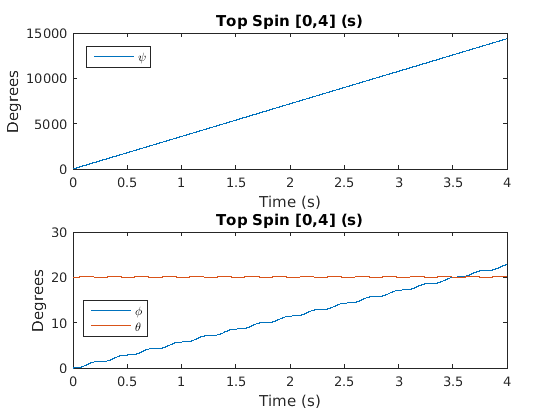
\includegraphics[width=1\textwidth]{../ex2/plots/forwardData.png}
	\caption{Showing the angle evolution for the spinning top problem over 4 seconds.}
	\label{fig:forwardData}
\end{figure}

\begin{figure}[H]
	\centering
	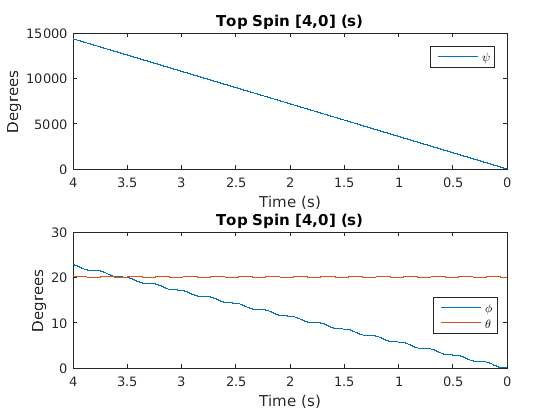
\includegraphics[width=1\textwidth]{../ex2/plots/backwardData.png}
	\caption{Showing the angle evolution for the spinning top problem when going backwards in time.}
	\label{fig:backwardData}
\end{figure}

\begin{figure}[H]
	\centering
	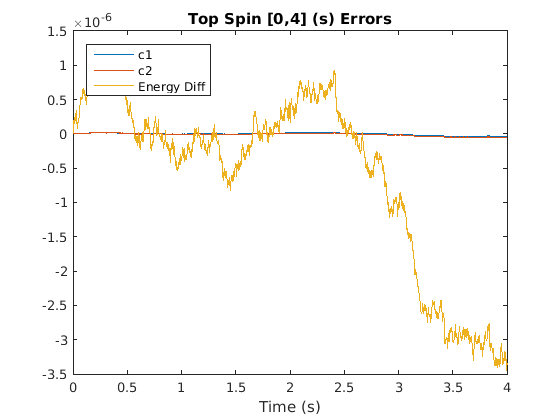
\includegraphics[width=1\textwidth]{../ex2/plots/forwardDataError.png}
	\caption{A zoom in on the error when stepping forwards in time.}
	\label{fig:forwardDataError}
\end{figure}

\begin{figure}[H]
	\centering
	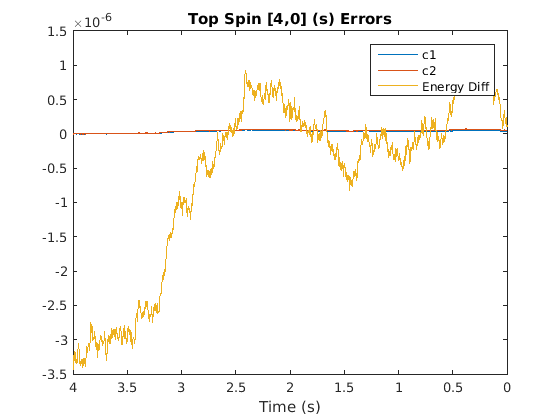
\includegraphics[width=1\textwidth]{../ex2/plots/backwardDataError.png}
	\caption{A zoom in on the error when stepping backwards in time.}
	\label{fig:backwardDataError}
\end{figure}

\begin{figure}[H]
	\centering
	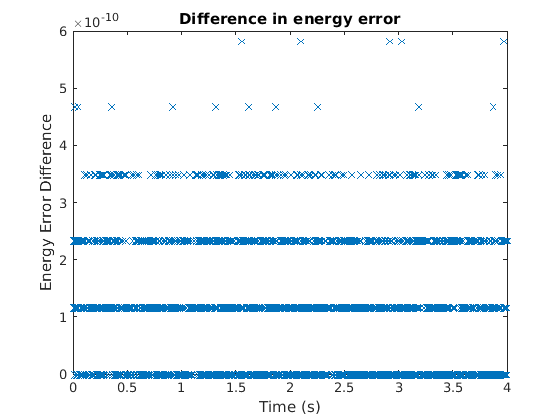
\includegraphics[width=1\textwidth]{../ex2/plots/energyErrorDiff.png}
	\caption{The error difference between forward and backward stepping through the solution.}
	\label{fig:energyErrorDiff}
\end{figure}

\section{Exercise 3}
In this exercise we start with deriving the Hamiltonian equations of motion from equation 29, 30 and 31 in the lab specification. We then end up with
\begin{align}
	\dot{\phi} &= \frac{ p_{\phi} -  p_{\psi} \cos{\theta}}{ I_1 \sin^2{\theta}} \\
	\dot{\psi} &= \frac{p_{\psi}}{I_3} - \frac{\cos{\theta}(p_{\phi}-p_{\psi}\cos{\theta}}{I_1 \sin^2{\theta}} \\
	\dot{\theta} &= \frac{p_{\theta}}{I_1} \\
	\dot{p_{\phi}} &= 0 \\
	\dot{p_{\psi}} &= 0 \\
	\dot{p_{\theta}} & = mgl\sin{\theta} - \frac{p_{\psi}(p_{\phi} - p_{\psi}\cos{\theta})}{I_1 \sin{\theta}} +\frac{\cos{\theta}(p_{\phi}-p_{\psi}\cos{\theta})^2}{I_1 \sin^3{\theta}}
\end{align}
The Jacobian, $J$, for a system like this will involve allot of zeros except for the following elements
\begin{align*}
J_{33} &=P_{\psi}^2/I_1 - mgl  \cos{\theta} + (P_{\phi} - P_{\psi}  \cos{\theta})^2/(I_1  \sin^2{\theta}) + \\
       &(3  \cos^2{\theta} (P_{\phi} - P_{\psi}  \cos{\theta})^2)/(I_1  \sin^4{\theta}) - \\
       &(3 P_{\psi}  \cos{\theta} (P_{\phi} - P_{\psi}  \cos{\theta}))/(I_1  \sin^2{\theta}) \\
J_{34} &=P_{\psi}/(I_1  \sin{\theta}) - ( \cos{\theta} (2 P_{\phi} - 2 P_{\psi}  \cos{\theta}))/(I_1  \sin^3{\theta}) \\
J_{35} &=(P_{\phi} - P_{\psi}  \cos{\theta})/(I_1  \sin{\theta}) - (P_{\psi}  \cos{\theta})/(I_1  \sin{\theta}) + \\
       &(2  \cos^2{\theta} (P_{\phi} - P_{\psi}  \cos{\theta}))/(I_1  \sin^3{\theta}) \\
J_{43} &=P_{\psi}/(I_1  \sin{\theta}) - ( \cos{\theta} (2 P_{\phi} - 2 P_{\psi}  \cos{\theta}))/(I_1  \sin^3{\theta}) \\
J_{44} &=1/(I_1  \sin^2{\theta}) \\
J_{45} &=- \cos{\theta}/(I_1  \sin^2{\theta}) \\
J_{53} &=(P_{\phi} - P_{\psi}  \cos{\theta})/(I_1  \sin{\theta}) - (P_{\psi}  \cos{\theta})/(I_1  \sin{\theta}) + \\
       &(2  \cos^2{\theta} (P_{\phi} - P_{\psi}  \cos{\theta}))/(I_1  \sin^3{\theta}) \\
J_{54} &=- \cos{\theta}/(I_1  \sin^2{\theta}) \\
J_{55} &=1/I_3 +  \cos^2{\theta}/(I_1  \sin^2{\theta}) \\
J_{66} &=1/I_1
\end{align*}
This was calculated by looking at the $\dot{\phi},\dot{\psi},\dot{\theta},\dot{P}_{\phi},\dot{P}_{\psi},\dot{P}_{\theta}$ functions with respect to ${\phi},{\psi},{\theta},{P}_{\phi},{P}_{\psi},{P}_{\theta}$.
\subsection{Running the Code}
To run the code simply run the \verb+make+ command inside the directory 
\begin{verbatim}
~jeve0010/Documents/jesper/fnm/lab3/ex3
\end{verbatim}
 then run the program with the command \verb+./ex3+. If one wants to obtain the plots showed in this document simply execute the matlab script 
\begin{verbatim}
 ~jeve0010/Documents/jesper/fnm/lab3/ex2/plots/code/topSpinHam.m.
\end{verbatim}

\subsection{Results and analysis}
Here we have done the same simulation of the spinning top as in the previous exercise, but using the Hamiltonian equations instead of the Lagrangian. We have used the same step sizes and initial values in order to get a proper comparison. One difference though is that we use a Runge-Kutta 45  stepping method for the Lagrangian and the Bulirsch-Stoer stepping method for the Hamiltonian equations. The resulting angles seem to be basically the same, which is encouraging. What is left then is the errors and how they react when we go backwards. First off we can see that the Hamiltonian equations gives an error that is two orders of magnitude smaller then what the Lagrangian equations did, this can easily be seen by comparing figure \ref{fig:forwardDataError} and \ref{fig:backwardDataError} with \ref{fig:forwardDataErrorHAM} and \ref{fig:backwardDataHAM}. This is a clear advantage to the Hamiltonian equations. We can also see in figure \ref{fig:energyErrorDiff} and \ref{fig:energyErrorDiffHAM} that the Hamiltonian equations yields a less deviating result when stepping backwards in the solution. These graphs displaying the difference in energy error also exhibit interesting discrete value differences, and there are fewer for the Hamiltonian equation. This could be taken as the Hamiltonian equations results in a problem that are more stable. But to be sure about that one has to know why the changes are discrete, and sadly the author can not figure out why. The step in between is seemingly larger then machine epsilon... So it maybe it could be the result of the solver and its numerical properties. We can also see that the momentum $P_{\phi}$ and $P_{\psi}$ are completely conserved in figure \ref{fig:forwardDataError}. Lastly one should note it took significant more time to solve with the Hamiltonian equations compared to the Lagrangian. With the Lagrangian equations it only took 2,542 seconds, compared to the Hamiltonian equations which took 1 minute and 32.072 seconds. That is a quite significant difference, but could be due to the stepping method used.

To conclude we can say that for this particular problem is that the Lagrangian equations with the Runge-Kutta stepping method is probably better just because of being hugely more effective to solve then using the Hamiltonian equations with the Bulirsch-Stoer stepping method. The Hamiltonian equations gave less error and where stabler, but only marginally. 
\begin{figure}[H]
	\centering
	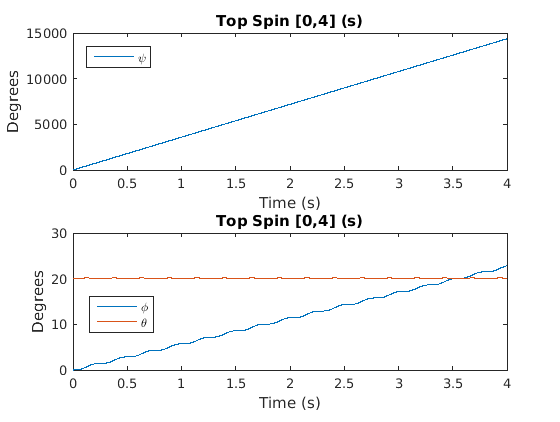
\includegraphics[width=1\textwidth]{../ex3/plots/forwardData.png}
	\caption{Showing the angle evolution for the spinning top problem over 4 seconds.}
	\label{fig:forwardDataHAM}
\end{figure}

\begin{figure}[H]
	\centering
	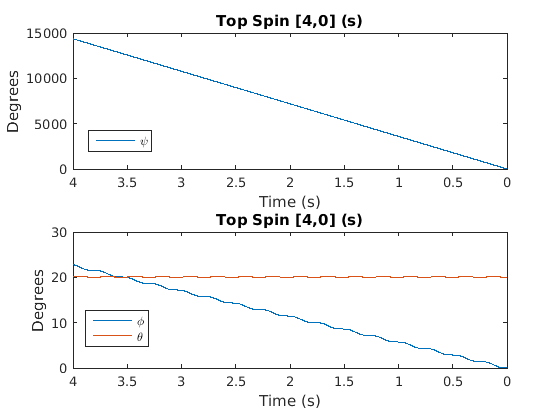
\includegraphics[width=1\textwidth]{../ex3/plots/backwardData.png}
	\caption{Showing the angle evolution for the spinning top problem when going backwards in time.}
	\label{fig:backwardDataHAM}
\end{figure}

\begin{figure}[H]
	\centering
	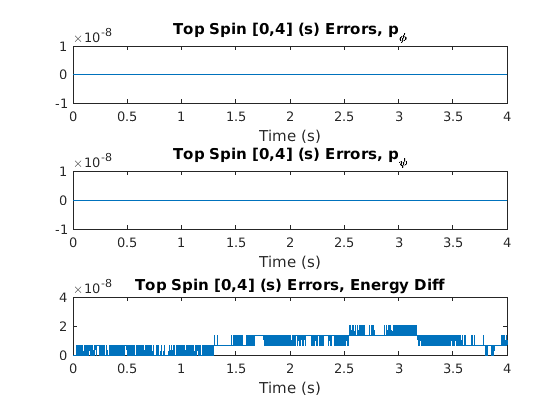
\includegraphics[width=1\textwidth]{../ex3/plots/forwardDataError.png}
	\caption{The errors stay at zero with eight decimals accuracy when stepping forwards in time. We have showed how much deviation occurs between the different values of $P_{\phi}, P_{\psi}$ and the energy of the system between steps.}
	\label{fig:forwardDataErrorHAM}
\end{figure}

\begin{figure}[H]
	\centering
	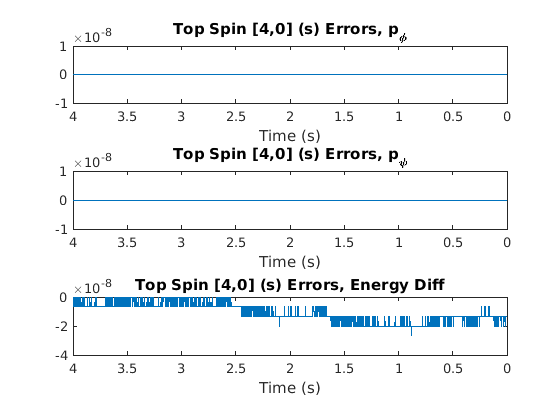
\includegraphics[width=1\textwidth]{../ex3/plots/backwardDataError.png}
	\caption{The errors stay at zero with eight decimals accuracy when stepping forwards in. We have showed how much deviation occurs between the different values of $P_{\phi}, P_{\psi}$ and the energy of the system between steps.}
	\label{fig:backwardDataErrorHAM}
\end{figure}

\begin{figure}[H]
	\centering
	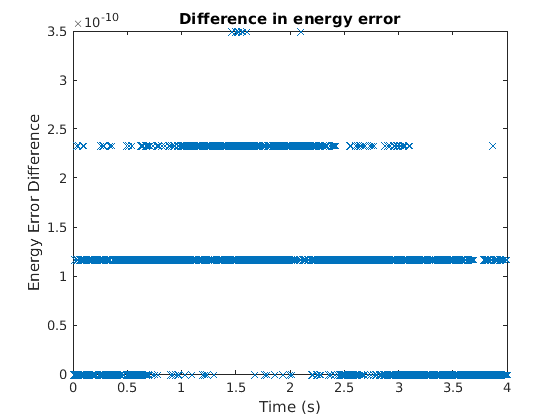
\includegraphics[width=1\textwidth]{../ex3/plots/energyErrorDiff.png}
	\caption{The error difference between forward and backward stepping through the solution.}
	\label{fig:energyErrorDiffHAM}
\end{figure}




\end{document}
